\documentclass[aspectratio=169, 10pt]{beamer}

% Theme & Styling
\usetheme{Madrid}
\usecolortheme{whale}

% Essential Packages
\usepackage{amsmath,amssymb}
\usepackage{booktabs}
\usepackage{graphicx}
\usepackage{xcolor}
\usepackage{microtype}
\usepackage{tikz}
\usetikzlibrary{shapes.geometric, arrows.meta, positioning}

% Custom Color Palette
\definecolor{primaryblue}{RGB}{0, 51, 153}
\definecolor{accentblue}{RGB}{41, 128, 185}
\definecolor{darknavy}{RGB}{20, 30, 55}
\definecolor{lightgraybg}{RGB}{245, 247, 250}

\setbeamercolor{palette primary}{bg=primaryblue, fg=white}
\setbeamercolor{palette secondary}{bg=accentblue, fg=white}
\setbeamercolor{palette tertiary}{bg=darknavy, fg=white}
\setbeamercolor{structure}{fg=primaryblue}
\setbeamercolor{title}{bg=primaryblue, fg=white}

% Navigation & Footer setup
\setbeamertemplate{navigation symbols}{}
\setbeamertemplate{footline}[frame number]

% Presentation Metadata
\title[\textbf{SecureNet IDS}]{\textbf{SecureNet IDS: A Hybrid Real-Time Network Intrusion Detection System}}
\subtitle{Integrating AI/ML with Multi-Source Threat Intelligence}

\author[SecureNet IDS Team]{
    \textbf{SecureNet IDS Team} \\[0.12cm]
    Anubhav Singh \quad -- \quad Kaushal Singh \\[0.08cm]
    Prasoon Pathak \quad -- \quad Prakhar Chaubey \\[0.25cm]
    \textit{Under the Guidance of:} \\
    \textbf{Ms. Sonali Kumari} (Assistant Professor)
}

\institute[CSE, UIT]{
    \textbf{Department of Computer Science and Engineering} \\
    \textbf{United Institute Of Technology}, Naini, Prayagraj \\
    \vspace{0.1cm}
    \small \textbf{Live Demo:} \url{https://secure-net-ids.vercel.app/} \quad $\vert$ \quad \textbf{Code:} \url{https://github.com/pathakpk7/SecureNet_IDS.git}
}

\date{Academic Session 2025--2026}

\begin{document}

% ==============================================================================
% SLIDE 1: TITLE SLIDE
% ==============================================================================
\begin{frame}[plain]
    \titlepage
\end{frame}

% ==============================================================================
% SLIDE 2: MOTIVATION & PROBLEM STATEMENT
% ==============================================================================
\begin{frame}{1. Motivation \& Problem Statement}
    \begin{columns}
        \begin{column}{0.5\textwidth}
            \textbf{Industry Context \& Challenges:}
            \begin{itemize}
                \item Rapid expansion of enterprise networks and cloud infrastructure against automated cyber attacks.
                \item \textbf{Signature-based IDS (Snort/Suricata)} fail to catch zero-day exploits and polymorphic malware.
                \item \textbf{Standalone ML Detectors} suffer from high false alarm rates and lack real-world threat attribution.
            \end{itemize}
        \end{column}
        \begin{column}{0.5\textwidth}
            \begin{block}{Project Objectives}
                \begin{enumerate}
                    \item Ingest packets and extract 5-tuple flow metrics at wire speed via Scapy/libpcap.
                    \item Train an optimized Random Forest achieving $>99\%$ accuracy with low latency.
                    \item Synthesize multi-source threat intelligence (AbuseIPDB + VirusTotal).
                    \item Execute automated host containment (null-routing, WAF rules, AI Copilot).
                \end{enumerate}
            \end{block}
        \end{column}
    \end{columns}
\end{frame}

% ==============================================================================
% SLIDE 3: SYSTEM ARCHITECTURE OVERVIEW
% ==============================================================================
\begin{frame}{2. System Architecture Overview}
    \centering
    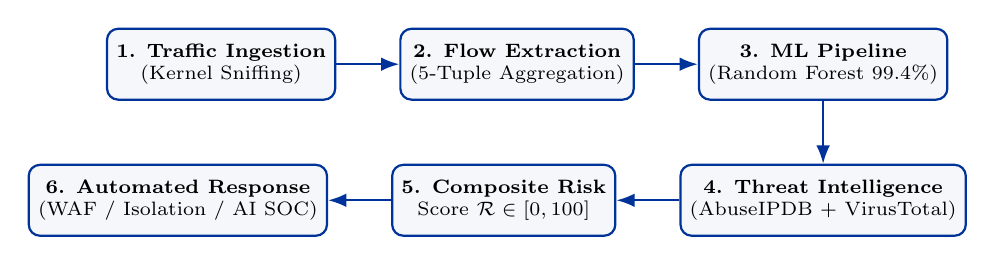
\begin{tikzpicture}[
        node distance=0.6cm and 0.8cm,
        box/.style={rectangle, draw=primaryblue, fill=lightgraybg, thick, rounded corners, align=center, font=\scriptsize, minimum height=0.9cm, minimum width=2.1cm},
        arrow/.style={-Latex, thick, primaryblue}
    ]
        \node[box] (ingest) {\textbf{1. Traffic Ingestion}\\(Kernel Sniffing)};
        \node[box, right=of ingest] (extract) {\textbf{2. Flow Extraction}\\(5-Tuple Aggregation)};
        \node[box, right=of extract] (ml) {\textbf{3. ML Pipeline}\\(Random Forest 99.4\%)};
        \node[box, below=0.8cm of ml] (ti) {\textbf{4. Threat Intelligence}\\(AbuseIPDB + VirusTotal)};
        \node[box, left=of ti] (score) {\textbf{5. Composite Risk}\\Score $\mathcal{R} \in [0, 100]$};
        \node[box, left=of score] (soc) {\textbf{6. Automated Response}\\(WAF / Isolation / AI SOC)};

        \draw[arrow] (ingest) -- (extract);
        \draw[arrow] (extract) -- (ml);
        \draw[arrow] (ml) -- (ti);
        \draw[arrow] (ti) -- (score);
        \draw[arrow] (score) -- (soc);
    \end{tikzpicture}
    
    \vspace{0.4cm}
    \begin{itemize}
        \item \textbf{Bidirectional 5-Tuple Key:} $\langle \text{IP}_{\text{src}},\, \text{IP}_{\text{dst}},\, \text{Port}_{\text{src}},\, \text{Port}_{\text{dst}},\, \text{Proto} \rangle$
        \item \textbf{Continuous Tracking:} IAT, forward/backward counts, byte volumes, TCP flags (SYN, ACK, RST).
    \end{itemize}
\end{frame}

% ==============================================================================
% SLIDE 4: DFD LEVEL 0 (CONTEXT DIAGRAM)
% ==============================================================================
\begin{frame}{3. Data Flow Diagram: Level 0 (Context Diagram)}
    \centering
    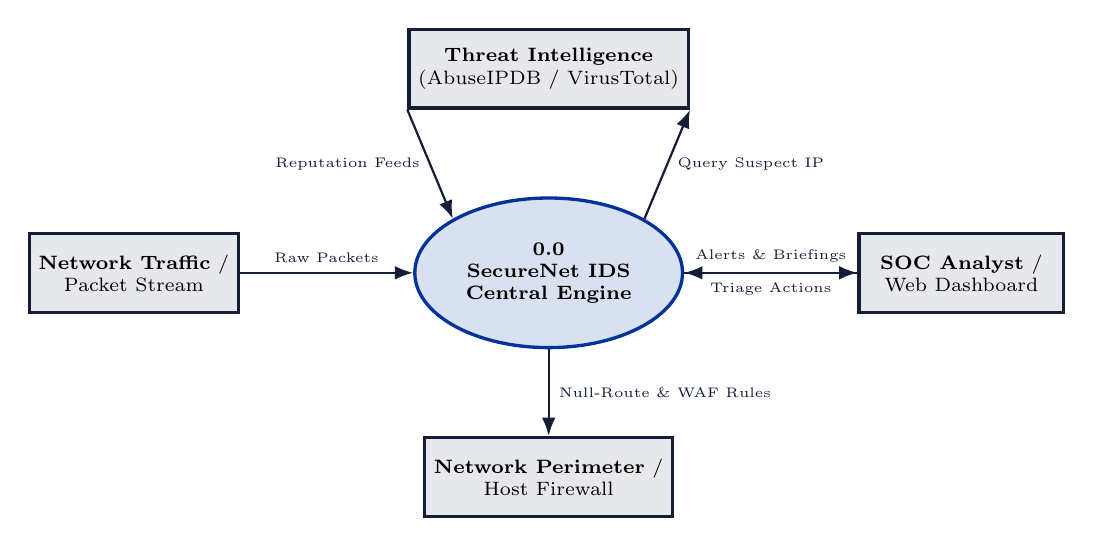
\begin{tikzpicture}[
        entity/.style={rectangle, draw=darknavy, fill=darknavy!10, very thick, minimum width=2.6cm, minimum height=1.0cm, align=center, font=\scriptsize},
        process/.style={ellipse, draw=primaryblue, fill=primaryblue!15, very thick, minimum width=3.4cm, minimum height=1.9cm, align=center, font=\scriptsize},
        arrow/.style={-{Latex[scale=1]}, thick, color=darknavy, font=\tiny}
    ]
        \node[process] (p0) {\textbf{0.0}\\\textbf{SecureNet IDS}\\\textbf{Central Engine}};
        \node[entity, left=2.2cm of p0] (traffic) {\textbf{Network Traffic} /\\Packet Stream};
        \node[entity, above=1.1cm of p0] (threatintel) {\textbf{Threat Intelligence}\\(AbuseIPDB / VirusTotal)};
        \node[entity, right=2.2cm of p0] (soc) {\textbf{SOC Analyst} /\\Web Dashboard};
        \node[entity, below=1.1cm of p0] (firewall) {\textbf{Network Perimeter} /\\Host Firewall};

        \draw[arrow] (traffic) -- node[above] {Raw Packets} (p0);
        \draw[arrow] (p0.north east) -- node[right] {Query Suspect IP} (threatintel.south east);
        \draw[arrow] (threatintel.south west) -- node[left] {Reputation Feeds} (p0.north west);
        \draw[arrow] (p0) -- node[above] {Alerts \& Briefings} (soc);
        \draw[arrow] (soc) -- node[below] {Triage Actions} (p0);
        \draw[arrow] (p0) -- node[right] {Null-Route \& WAF Rules} (firewall);
    \end{tikzpicture}
\end{frame}

% ==============================================================================
% SLIDE 5: DFD LEVEL 1 (SUBSYSTEM DECOMPOSITION)
% ==============================================================================
\begin{frame}{4. Data Flow Diagram: Level 1 (Subsystem Decomposition)}
    \centering
    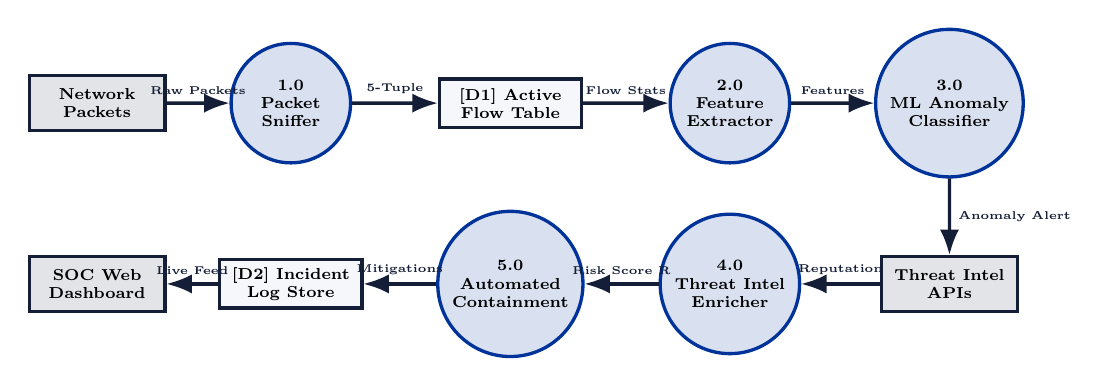
\begin{tikzpicture}[
        scale=0.82, transform shape,
        proc/.style={circle, draw=primaryblue, fill=primaryblue!15, very thick, minimum size=1.85cm, align=center, font=\scriptsize\bfseries},
        store/.style={rectangle, draw=darknavy, fill=lightgraybg, very thick, minimum width=2.2cm, minimum height=0.75cm, align=center, font=\scriptsize\bfseries},
        entity/.style={rectangle, draw=darknavy, fill=darknavy!12, very thick, minimum width=2.1cm, minimum height=0.85cm, align=center, font=\scriptsize\bfseries},
        arrow/.style={-{Latex[scale=1.1]}, very thick, color=darknavy, font=\tiny\bfseries}
    ]
        % Top Row
        \node[entity] (net) at (0, 3.2) {Network\\Packets};
        \node[proc] (p1) at (3.0, 3.2) {1.0\\Packet\\Sniffer};
        \node[store] (d1) at (6.4, 3.2) {[D1] Active\\Flow Table};
        \node[proc] (p2) at (9.8, 3.2) {2.0\\Feature\\Extractor};
        \node[proc] (p3) at (13.2, 3.2) {3.0\\ML Anomaly\\Classifier};

        % Bottom Row
        \node[entity] (ti) at (13.2, 0.4) {Threat Intel\\APIs};
        \node[proc] (p4) at (9.8, 0.4) {4.0\\Threat Intel\\Enricher};
        \node[proc] (p5) at (6.4, 0.4) {5.0\\Automated\\Containment};
        \node[store] (d2) at (3.0, 0.4) {[D2] Incident\\Log Store};
        \node[entity] (soc) at (0, 0.4) {SOC Web\\Dashboard};

        % Connections
        \draw[arrow] (net) -- node[above] {Raw Packets} (p1);
        \draw[arrow] (p1) -- node[above] {5-Tuple} (d1);
        \draw[arrow] (d1) -- node[above] {Flow Stats} (p2);
        \draw[arrow] (p2) -- node[above] {Features} (p3);
        \draw[arrow] (p3) -- node[right] {Anomaly Alert} (ti);
        \draw[arrow] (ti) -- node[above] {Reputation} (p4);
        \draw[arrow] (p4) -- node[above] {Risk Score R} (p5);
        \draw[arrow] (p5) -- node[above] {Mitigations} (d2);
        \draw[arrow] (d2) -- node[above] {Live Feed} (soc);
    \end{tikzpicture}
\end{frame}

% ==============================================================================
% SLIDE 6: DFD LEVEL 2 (PERFECT SPACING, NO COLLISION, CLEAN BUS)
% ==============================================================================
\begin{frame}{5. Data Flow Diagram: Level 2 (Inference \& Containment Subsystem)}
    \centering
    \vspace{-0.1cm}
    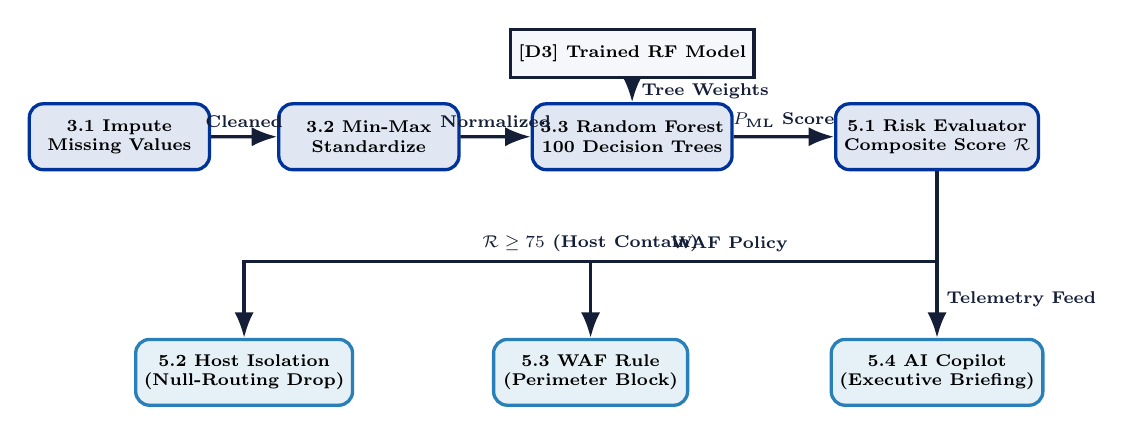
\begin{tikzpicture}[
        scale=0.88, transform shape,
        proc/.style={rectangle, draw=primaryblue, fill=primaryblue!12, rounded corners=5pt, very thick, minimum width=2.6cm, minimum height=0.95cm, align=center, font=\scriptsize\bfseries},
        store/.style={rectangle, draw=darknavy, fill=lightgraybg, very thick, minimum width=2.4cm, minimum height=0.7cm, align=center, font=\scriptsize\bfseries},
        action/.style={rectangle, draw=accentblue, fill=accentblue!12, rounded corners=5pt, very thick, minimum width=2.8cm, minimum height=0.95cm, align=center, font=\scriptsize\bfseries},
        arrow/.style={-{Latex[scale=1.1]}, very thick, color=darknavy, font=\scriptsize\bfseries}
    ]
        % Stage 3: ML Pipeline (Upper Row)
        \node[proc] (p31) at (0.2, 3.8) {3.1 Impute\\Missing Values};
        \node[proc] (p32) at (3.8, 3.8) {3.2 Min-Max\\Standardize};
        \node[proc] (p33) at (7.6, 3.8) {3.3 Random Forest\\100 Decision Trees};
        \node[store] (rfmodel) at (7.6, 5.0) {[D3] Trained RF Model};
        \node[proc] (p51) at (12.0, 3.8) {5.1 Risk Evaluator\\Composite Score $\mathcal{R}$};

        % Stage 5: Response Actions (Lower Row - Clean 3 Columns)
        \node[action] (nullroute) at (2.0, 0.4) {5.2 Host Isolation\\(Null-Routing Drop)};
        \node[action] (waf) at (7.0, 0.4) {5.3 WAF Rule\\(Perimeter Block)};
        \node[action] (copilot) at (12.0, 0.4) {5.4 AI Copilot\\(Executive Briefing)};

        % Upper ML Connections
        \draw[arrow] (p31) -- node[above] {Cleaned} (p32);
        \draw[arrow] (p32) -- node[above] {Normalized} (p33);
        \draw[arrow] (rfmodel) -- node[right] {Tree Weights} (p33);
        \draw[arrow] (p33) -- node[above] {$P_{\text{ML}}$ Score} (p51);

        % Distribution Bus (Clean horizontal conduit, NO crossing lines)
        \coordinate (bus) at (12.0, 2.0);
        \draw[very thick, color=darknavy] (p51.south) -- (bus);
        
        % Branches dropping from bus to action nodes
        \draw[arrow] (bus) -| node[above, pos=0.25] {$\mathcal{R} \ge 75$ (Host Contain)} (nullroute.north);
        \draw[arrow] (bus) -| node[above, pos=0.3] {WAF Policy} (waf.north);
        \draw[arrow] (bus) -- node[right] {Telemetry Feed} (copilot.north);
    \end{tikzpicture}
\end{frame}

% ==============================================================================
% SLIDE 7: THREAT SCORING & INCIDENT RESPONSE
% ==============================================================================
\begin{frame}{6. Composite Threat Scoring \& Response Playbooks}
    \begin{block}{Composite Risk Score Formulation}
        $$\mathcal{R} = w_1 \cdot P_{\text{ML}} + w_2 \cdot S_{\text{Abuse}} + w_3 \cdot S_{\text{VT}}$$
        \small Where $w_1 = 0.45$ (ML anomaly confidence), $w_2 = 0.35$ (AbuseIPDB abuse score), and $w_3 = 0.20$ (VirusTotal reputation).
    \end{block}

    \vspace{0.2cm}
    \textbf{Automated Incident Containment Playbooks (NIST SP 800-31 Aligned):}
    \begin{itemize}
        \item \textbf{Low Severity ($\mathcal{R} < 40$):} Background audit logging; continuous passive telemetry tracking.
        \item \textbf{Medium Severity ($40 \le \mathcal{R} < 75$):} Rate-limiting enabled; IP marked for active SOC investigation.
        \item \textbf{Critical Severity ($\mathcal{R} \ge 75$):} Immediate automatic mitigation activated:
        \begin{enumerate}
            \item \emph{Host Isolation:} Automated insertion of null-route drops in OS routing tables.
            \item \emph{WAF Filtering:} Synthesis of blocking perimeter rules for web attacks.
            \item \emph{Forensic PCAP:} Extraction of raw suspicious traffic buffer for audit trail.
        \end{enumerate}
    \end{itemize}
\end{frame}

% ==============================================================================
% SLIDE 8: EXPERIMENTAL RESULTS & LATENCY
% ==============================================================================
\begin{frame}{7. Experimental Results \& System Performance}
    \begin{columns}
        \begin{column}{0.54\textwidth}
            \textbf{Model Evaluation (NSL-KDD \& Live Traffic):}
            \vspace{0.1cm}
            \begin{table}[h]
                \centering
                \scriptsize
                \begin{tabular}{lcccc}
                    \toprule
                    \textbf{Model} & \textbf{Acc.} & \textbf{Prec.} & \textbf{Recall} & \textbf{F1} \\
                    \midrule
                    Logistic Reg. & 88.6\% & 0.871 & 0.894 & 0.882 \\
                    KNN & 92.4\% & 0.915 & 0.928 & 0.921 \\
                    SVM & 94.2\% & 0.938 & 0.945 & 0.941 \\
                    Decision Tree & 96.8\% & 0.962 & 0.971 & 0.966 \\
                    \textbf{Random Forest} & \textbf{99.4\%} & \textbf{0.992} & \textbf{0.995} & \textbf{0.993} \\
                    \bottomrule
                \end{tabular}
            \end{table}
        \end{column}
        \begin{column}{0.46\textwidth}
            \textbf{Processing Latency Breakdown:}
            \vspace{0.1cm}
            \begin{table}[h]
                \centering
                \scriptsize
                \begin{tabular}{lcc}
                    \toprule
                    \textbf{Pipeline Stage} & \textbf{Latency} & \textbf{CPU} \\
                    \midrule
                    Packet Sniffing & 2.15 ms & 4.2\% \\
                    Flow Extraction & 6.05 ms & 8.5\% \\
                    RF Inference & 2.95 ms & 5.8\% \\
                    Composite Scoring & 0.35 ms & 0.8\% \\
                    \midrule
                    \textbf{Total Turnaround} & \textbf{11.90 ms} & \textbf{20.4\%} \\
                    \bottomrule
                \end{tabular}
            \end{table}
        \end{column}
    \end{columns}
    \vspace{0.3cm}
    \begin{itemize}
        \item \textbf{Sub-12 ms turnaround} comfortably supports live departmental campus network throughput.
        \item Low compute footprint enables deployment on standard edge servers without GPU cards.
    \end{itemize}
\end{frame}

% ==============================================================================
% SLIDE 9: LIVE SYSTEM DEPLOYMENT
% ==============================================================================
\begin{frame}{8. Live Deployment \& SOC Copilot}
    \begin{columns}
        \begin{column}{0.55\textwidth}
            \textbf{Operational Features:}
            \begin{itemize}
                \item Real-time Web Dashboard (Responsive Laptop \& Mobile UI).
                \item Live attack frequency charts \& threat vector distributions.
                \item \textbf{AI SOC Copilot:} Interactive natural language explanations of alerts \& containment recommendations.
                \item One-click response execution (WAF, PCAP, Host Isolation).
            \end{itemize}
            
            \vspace{0.2cm}
            \textbf{Live Links:}
            \begin{itemize}
                \item \textbf{Live App:} \url{https://secure-net-ids.vercel.app/}
                \item \textbf{GitHub:} \url{https://github.com/pathakpk7/SecureNet_IDS.git}
            \end{itemize}
        \end{column}
        \begin{column}{0.45\textwidth}
            \begin{exampleblock}{Impact \& Novelty}
                SecureNet IDS transforms static IDS logs into an automated detection-to-containment loop, dramatically cutting MTTR (Mean Time to Respond) from minutes to milliseconds.
            \end{exampleblock}
        \end{column}
    \end{columns}
\end{frame}

% ==============================================================================
% SLIDE 10: CONCLUSION & FUTURE WORK
% ==============================================================================
\begin{frame}{9. Conclusion \& Future Roadmap}
    \textbf{Key Project Achievements:}
    \begin{itemize}
        \item Developed an enterprise-ready hybrid network intrusion detection system.
        \item Achieved \textbf{99.42\% classification accuracy} with sub-12 ms latency on standard CPUs.
        \item Suppressed false-alarm alert fatigue by enriching alerts with AbuseIPDB \& VirusTotal feeds.
        \item Automated response playbooks and integrated an interactive AI SOC Security Copilot.
    \end{itemize}

    \vspace{0.3cm}
    \textbf{Future Enhancements:}
    \begin{itemize}
        \item Kernel-level eBPF/XDP drivers for multi-gigabit throughput.
        \item Graph Neural Networks (GNN) to track internal lateral movement.
        \item Quantized local on-premise LLMs for zero-leakage SOC telemetry analysis.
    \end{itemize}
    
    \vspace{0.4cm}
    \centering
    {\large \textbf{\color{primaryblue} Thank You! Questions \& Discussion}}
\end{frame}

\end{document}
